\begin{figure}[ht]
  \centering
  \begin{subfigure}[h]{0.4\linewidth}
    \centering
    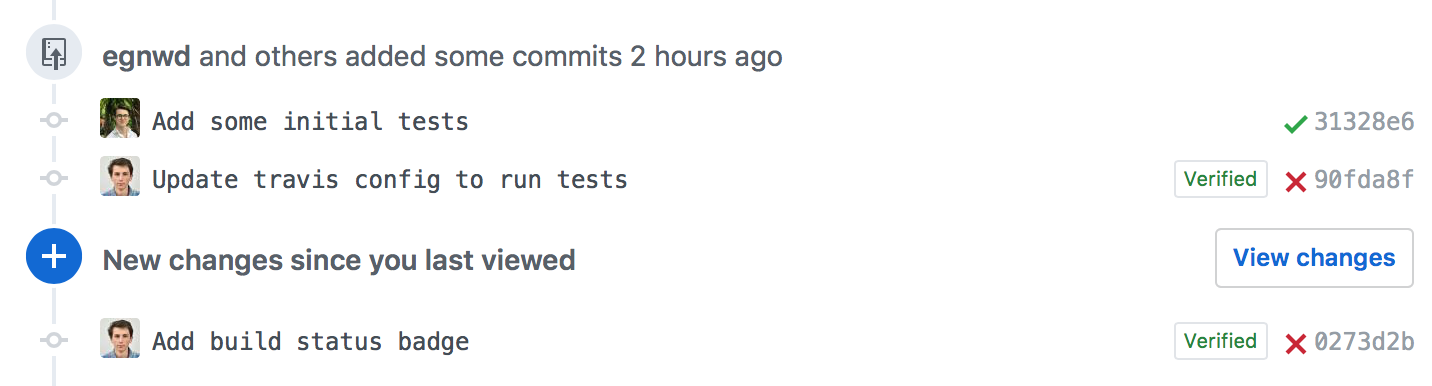
\includegraphics[width=\linewidth]{ci-1.png}
    \caption{Shows build status of commits within the code review}
    \label{fig:ci-1}
  \end{subfigure}
  \hfill
  \begin{subfigure}[h]{0.4\linewidth}
    \centering
    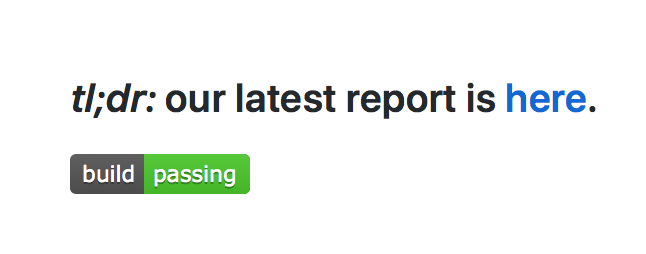
\includegraphics[width=\linewidth]{ci-2.png}
    \caption{Our git repo homepage shows us the current state of master}
    \label{fig:ci-2}
  \end{subfigure}
  \\
  \begin{subfigure}[h]{0.4\linewidth}
    \centering
    
\includegraphics[width=\linewidth]{ci-3.png}
    \caption{Tests help us avoid embarassing mistakes, e.g.~the wrong title}
    \label{fig:ci-3}
  \end{subfigure}
  \hfill
  \begin{subfigure}[h]{0.4\linewidth}
    \centering
    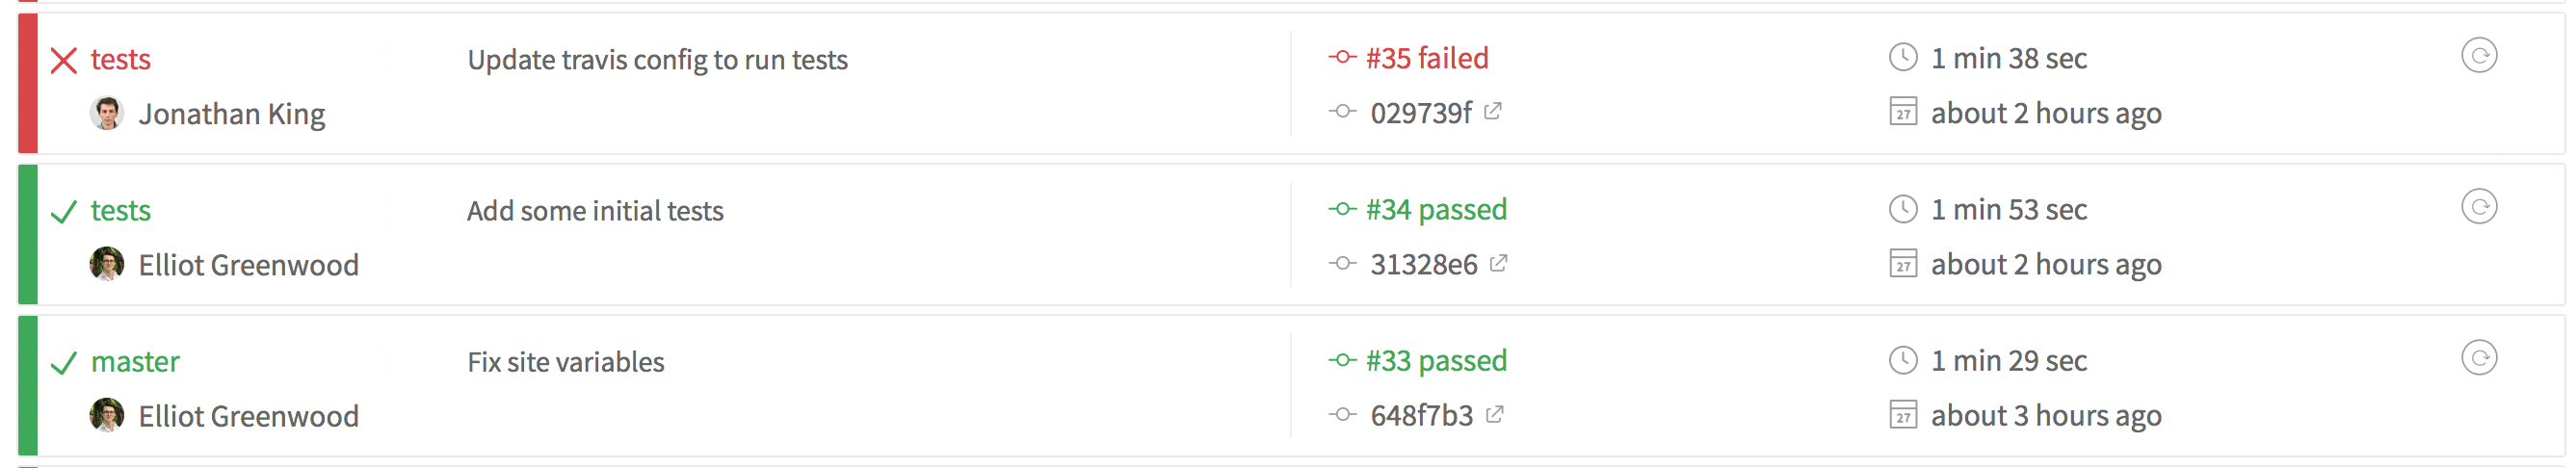
\includegraphics[width=\linewidth]{ci-4.png}
    \caption{Clear build log of builds and releases}
    \label{fig:ci-4}
  \end{subfigure}
  \caption{Screenshots of our build pipeline}
  \label{fig:}
\end{figure}
